% Chapter 1
\chapter{Mesure de la Durabilité dans le Développement Logiciel}	%The main chapter title
\label{mesure}
%%%%%%%%%%%%%%%%%%%%%%%%%%%%%%%%%%%%

Alors que la révolution technologique bat son plein, le génie logiciel se retrouve à la croisée des chemins en matière de durabilité. Ce premier chapitre explore l'intégration de la durabilité dans le développement logiciel, en soulignant les défis, les opportunités et les solutions qui se présentent à nous.


Divisé en trois parties distinctes, ce chapitre examine les aspects clés de la mesure de la durabilité dans le développement logiciel. La première section se concentre sur la conception d'un modèle de mesure complet capable d'évaluer la performance et la durabilité des projets logiciels (Section~\ref{sec:mesure-durabilite}). La deuxième section explore l'état de l'art des approches durables dans le domaine du génie logiciel, en les classifiant et en les évaluant dans un contexte en constante évolution (Section~\ref{sec:approches-durables}). La dernière section analyse les différentes dimensions de la durabilité conceptualisées dans la littérature académique en génie logiciel (Section~\ref{sec:dimensions-durabilite}).

%%%%%%%%%%%%%%%%%%%%%%%%%%%%%%%%%%%%

\section{Modèle de Mesure de la Performance et de Durabilité}\label{sec:mesure-durabilite}

%%%%%%%%%%%%%%%%%%%%%%%%%%%%%%%%%%%%

La mesure de la durabilité est au cœur de notre réflexion sur le génie logiciel durable. 
Pour comprendre comment intégrer efficacement la durabilité dans l'évaluation des performances des projets logiciels, nous débutons en explorant la création d'un modèle de mesure de la performance et de durabilité. Il représente un défi complexe qui nécessite une approche nuancée et multidimensionnelle. 
Plusieurs recherches ont offert des perspectives variées sur cette question cruciale.

\subsection{Approche et critères de mesure}
Le concept de logiciel vert, qui englobe les logiciels respectueux de l'environnement et économes en ressources, est de plus en plus présent dans le paysage contemporain du développement logiciel. Selon les auteurs du journal The GREENSOFT Model, \emph{« producing ecologically sound, resource and energy efficient software is also an issue nowadays »}~\cite{GreenSoftModel}. Cependant, la mesure et l'évaluation de la durabilité des processus de développement de logiciels et des produits logiciels qui en résultent restent un défi.


Pour répondre à ce défi, ces mêmes auteurs proposent \emph{« Appropriate criteria and metrics may comprise models for the measurement of software quality, procedure models for software development, as well as methods borrowed from LCA. Here, we distinguish direct criteria and metrics (related to first-order effects) from those which indirectly concern sustainability (related to second- and third-order effects) »}~\cite{GreenSoftModel}. Ainsi, il est décisif de disposer de cadres globaux qui prennent en compte d'une part les mesures directes et quantifiables de la consommation de ressources et des économies d'énergie, d'autre part les effets indirects sur la durabilité à long terme.


De plus, la prévalence des discussions sur l'efficacité énergétique au sein de la communauté des chercheurs suggère une prise de conscience croissante de l'impact environnemental du développement de logiciels. Dans l'article Green and Sustainable Software Engineering, il est indiqué que \emph{« Several approaches discussed efficiency in terms of energy consumption. This evidence may indicate the need to consider energy efficiency as an important quality attribute when designing systems architectures »}~\cite{GreenSustainableEngMapping}. Il est donc important d'intégrer des considérations de durabilité tout au long du cycle de vie du développement logiciel, de la conception et de l'architecture à la mise en œuvre et à la maintenance.


Enfin, en adoptant une approche multidimensionnelle et des critères de mesure rigoureux, l'industrie du développement logiciel peut s'efforcer de créer des logiciels non seulement fonctionnels et fiables, mais aussi écologiquement responsables et contribuant à un avenir durable. Il existe déjà des efforts importants pour atteindre cet objectif : \emph{« We observed that 56\% of the primary studies proposed means to achieve the energy efficiency of the software in terms of consumption and energy savings »}~\cite{GreenSustainableEngMapping}.

\begin{figure}[H]
    \centering
    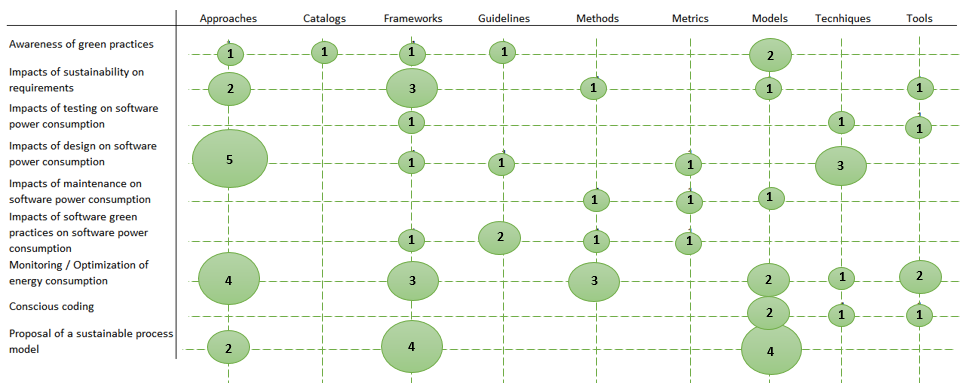
\includegraphics[width=1\textwidth]{MemoireMaster-NestorSkoczylas/figures/Répartition des études primaires selon les modèles de produits et processus proposés.png}
    \caption{Répartition des études primaires selon les modèles de produits et processus proposés}
    \label{fig:repartition-etudes-primaires}
\end{figure}

Comme le montre la Figure \ref{fig:repartition-etudes-primaires}, la plupart des études se concentrent sur les modèles de produits (approches, frameworks, etc.) pour le développement logiciel durable, tandis que les modèles de processus (13\%) sont moins étudiés. Parmi les rares modèles de processus proposés, seulement deux s'appuient sur des normes de qualité SE traditionnelles.

Ce manque de modèles de processus durables souligne la nécessité d'investir davantage dans ce domaine pour atteindre l'objectif d'un développement logiciel plus écologique. En effet, les modèles de processus guident les développeurs dans la création de logiciels économes en énergie et respectueux de l'environnement.

% Approach and measurement criteria
%~\cite{GreenSoftModel}	"Appropriate criteria and metrics may comprise models for the measurement of software quality, procedure models for software development, as well as methods borrowed from LCA. Here, we distinguish direct criteria and metrics (related to first-order effects) from those which indirectly concern sustainability (related to second- and third-order effects)."
%~\cite{GreenSoftModel}	"Appropriate criteria and metrics may comprise models for the measurement of software quality, procedure models for software development, as well as methods borrowed from LCA. Here, we distinguish direct criteria and metrics (related to first-order effects) from those which indirectly concern sustainability (related to second- and third-order effects)."
%~\cite{GreenSustainableEngMapping} "We observed that 56\% of the primary studies proposed means to achieve the energy efficiency of the software in terms of consumption and energy savings"
%~\cite{GreenSustainableEngMapping} "Several approaches discussed efficiency in terms of energy consumption. This evidence may indicate the need to consider energy efficiency as an important quality attribute when designing systems architectures."

\subsection{Intégrer des pratiques écologiques dans le \acrfull{sdlc}}
L'intégration efficiente de pratiques écologiques dans le \acrshort{sdlc} constitue un élément crucial pour atteindre un développement durable des logiciels. Bien que diverses approches et cadres soient disponibles, comme le souligne l'article~\cite{GreenSoftModel} : \emph{« Besides reflecting the proposed life cycle of a software product, there are further methods that support software architects, designers, and developers in producing green and sustainable software applications. »} Toutefois, des défis persistent pour intégrer harmonieusement ces pratiques avec les processus de développement existants.


Un aspect important à considérer réside dans la distinction entre les pratiques écologiques et les activités traditionnelles du \acrshort{sdlc}. L'article~\cite{GreenAgileMethods} affirme que : \emph{« The Sustainability Retrospective and the Sprint Retrospectives should not be combined, because they have a different timely position regarding the process flow and the focus »}, soulignant ainsi la nécessité de disposer de mécanismes distincts pour évaluer et améliorer la durabilité, en parallèle aux rétrospectives régulières du cycle de développement.


Selon l'article~\cite{GreenSustainableEngMapping} : \emph{« It was also possible to understand how sustainability has been addressed in the SLDC. The SMS shows that approaches and frameworks are mainly focused on the requirements and design phases. »} Cependant, la recherche actuelle suggère que la mise en œuvre des pratiques écologiques se limite souvent à ces premières étapes du \acrshort{sdlc}. Ce constat implique un besoin potentiel d'intégration plus large des aspects écologiques tout au long du cycle de développement, y compris les phases de mise en œuvre, de test, de déploiement et de maintenance.


Afin d'assurer une approche holistique et efficace pour atteindre les objectifs de développement de logiciels écologiques, une analyse approfondie des différences temporelles et fonctionnelles entre les pratiques écologiques et les activités traditionnelles du \acrshort{sdlc} s'avère nécessaire. En élargissant le champ d'intégration au-delà des phases initiales du développement, l'industrie du développement de logiciels peut garantir une approche plus globale et plus efficace pour atteindre les objectifs de développement de logiciels écologiques.

% Integration with the Software Development Life Cycle (SDLC)
%~\cite{GreenAgileMethods}	"The Sustainability Retrospective and the Sprint Retrospectives should not be combined, because they have a different timely position regarding the process flow and the focus."
%~\cite{GreenSoftModel}	"Besides reflecting the proposed life cycle of a software product, there are further methods that support software architects, designers, and developers in producing green and sustainable software applications."
%~\cite{GreenSustainableEngMapping} "It was also possible to understand how sustainability has been addressed in the SLDC. The SMS shows that approaches and frameworks are mainly focused on the requirements and design phases."

\subsection{Recherche et orientation futures}
Pour faire progresser le domaine de l'ingénierie logicielle écologique, une approche à multiples facettes est nécessaire, combinant recherche empirique et exploration des orientations futures. L'étude des perspectives des praticiens est essentielle pour comprendre les pratiques actuelles et identifier les domaines à améliorer. Selon~\cite{EmpiricalStudy} : \emph{« an analysis of the collected data that identifies practitioners’ perspectives on green software engineering throughout the software development process. »}


En s'appuyant sur cette base, des recherches plus approfondies peuvent contextualiser les connaissances existantes avec de nouveaux résultats.~\cite{EmpiricalStudy} propose \emph{« a discussion that contextualizes the state-of-the-art in green software engineering research with respect to the study’s findings, and suggests, for each stage of the software development process, directions for future green software engineering research. »} Cette approche synergique comble le fossé entre les connaissances théoriques et l'application pratique, conduisant à des pratiques de développement de logiciels écologiques plus efficaces et plus faciles à mettre en œuvre.


Il est important de souligner la nécessité d'un développement et d'une amélioration continus des différents aspects de l'ingénierie logicielle écologique.~\cite{GreenSustainableEngMapping} appuie cette idée en affirmant que : \emph{« There are several directions to follow towards establishing and improving Green SE practice, in particular in order to provide the SE practice with green and sustainability-aware processes, tools and methods. »} Ces orientations incluent la création de nouveaux outils et méthodologies, l'amélioration des processus existants et le développement de ressources éducatives pour doter les professionnels du logiciel des compétences et connaissances nécessaires pour concevoir, développer et maintenir des solutions logicielles durables.


La recherche empirique associé à une vision prospective, permet de tracer la voie vers un avenir où le développement de logiciels n'est pas seulement innovant et fonctionnel, mais également respectueux de l'environnement tout en contribuant à un avenir durable.

% Recherche et orientations futures
%~\cite{EmpiricalStudy}	"An analysis of the collected data that identifies practitioners’ perspectives on green software engineering throughout the software development process."
%~\cite{EmpiricalStudy}	"A discussion that contextualizes the state-of-the-art in green software engineering research with respect to the study’s findings, and suggests, for each stage of the software development process, directions for future green software engineering research."
%~\cite{GreenSustainableEngMapping} "There are several directions to follow towards establishing and improving Green SE practice, in particular in order to provide the SE practice with green and sustainability-aware processes, tools and methods."

\subsection{Modèles et théories existants}
Comprendre les modèles et théories existants est crucial pour enrichir la base de connaissances actuelle en matière de développement de logiciels écologiques. Ces modèles offrent des cadres pour conceptualiser la relation entre le développement de logiciels et la durabilité.


Le schéma illustrant la durabilité dans le génie logiciel (\ref{fig:durabilite-geni-logiciel}) présente une synthèse des principaux modèles et théories en matière de développement de logiciels durables. On peut y observer les différentes dimensions de la durabilité, ainsi que les relations entre elles.


Parmi ces modèles, le modèle GREENSOFT se distingue en mettant l'accent sur l'importance des critères et des mesures de durabilité (dimension économique de la figure \ref{fig:durabilite-geni-logiciel}).

Selon \cite{GreenSoftModel} : \emph{« The second part of the GREENSOFT Model is called Sustainability Criteria and Metrics. It covers common metrics and criteria for the measurement of software quality and it allows a classification of criteria and metrics for evaluating a software product’s sustainability. »} Il offre une approche structurée pour évaluer l'impact environnemental des produits logiciel.

\begin{figure}[H]
    \centering
    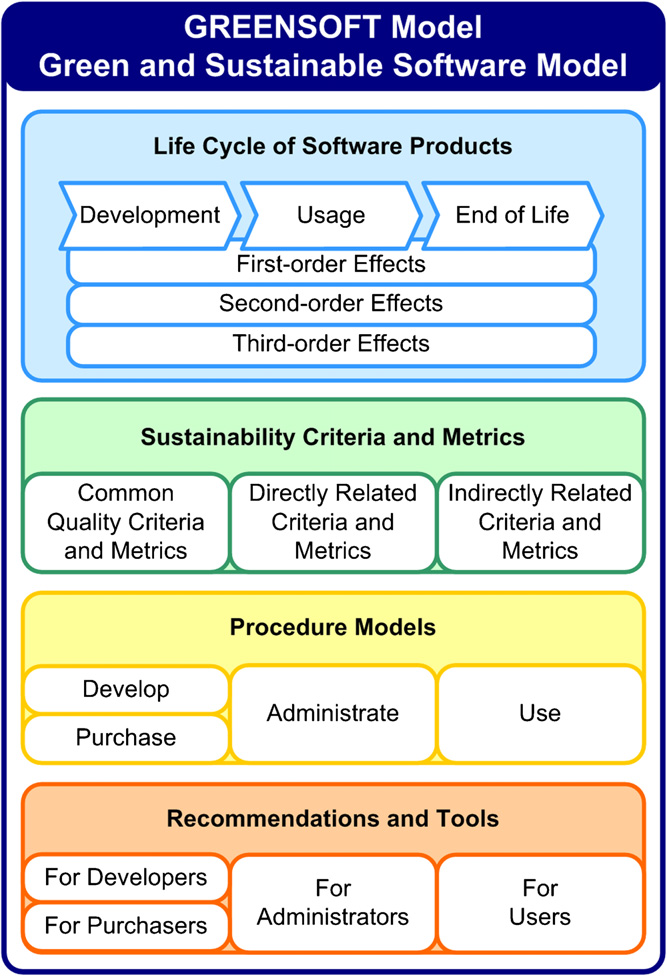
\includegraphics[width=0.4\textwidth]{MemoireMaster-NestorSkoczylas/figures/greensoft_model.png}
    \caption{Le modèle GREENSOFT}
    \label{fig:greensoft-model}
\end{figure}

La figure ci-dessus (\ref{fig:greensoft-model}) présente le modèle GREENSOFT. Le cycle de vie des produits logiciels est représenté au centre de la figure. Les trois phases du cycle de vie (développement, utilisation et fin de vie) sont représentées par des rectangles. Les autres éléments du modèle GREENSOFT (critères et métriques de durabilité, modèles de procédure, recommandations et outils) sont représentés autour du cycle de vie.

La théorie de la stratification durable, quant à elle, propose une perspective nuancée sur la relation entre le développement de logiciels et la durabilité (dimensions sociale et environnementale de la \ref{fig:durabilite-geni-logiciel}). Cette théorie, telle qu’elle est citée dans~\cite{SustainableStratifiedTheory}, \emph{« explain how sustainability relates to software development based on existing qualitative research and to provide a more nuanced view of the stratified and multisystemic nature of sustainability according to our observations from the meta-synthesis. »} En reconnaissant la nature complexe et interconnectée de la durabilité, cette théorie encourage une approche globale du développement de logiciels écologiques.


De plus, la théorie de la stratification durable met en évidence l'interdépendance des processus et des produits logiciels. Selon~\cite{SustainableStratifiedTheory} : \emph{« The model separates the software process from the software product to illustrate that sustainability is a property of both, and while the nature of the software development process affects the resulting software system, a sustainable process does not guarantee a sustainable product or vice versa. »} Cela souligne la nécessité de considérer les deux aspects en tandem lors du développement de logiciels durables.


En étudiant et en évaluant de manière critique les modèles et théories existants, la communauté des développeurs de logiciels peut acquérir des connaissances précieuses sur les complexités et les interrelations inhérentes à ce domaine. Ces connaissances peuvent ensuite servir de base à de nouveaux efforts de recherche et de développement, ouvrant ainsi la voie à un avenir plus durable en matière de développement de logiciels.

% Modèles et théories existants
%~\cite{GreenSoftModel}	"The second part of the GREENSOFT Model is called Sustainability Criteria and Metrics. It covers common metrics and criteria for the measurement of software quality [43] and it allows a classification of criteria and metrics for evaluating a software product’s sustainability."
%~\cite{SustainableStratifiedTheory} "The goal of this model is to explain how sustainability relates to software development based on existing qualitative research and to provide a more nuanced view of the stratified and multisystemic nature of sustainability according to our observations from the meta-synthesis."
%~\cite{SustainableStratifiedTheory} "The model separates the software process from the software product to illustrate that sustainability is a property of both, and while the nature of the software development process affects the resulting software system, a sustainable process does not guarantee a sustainable product or vice versa."

\paragraph{}
En guise de conclusion, l'élaboration d'un modèle de mesure de la performance et de la durabilité constitue un élément fondamental pour l'ingénierie logicielle durable. Cette tâche ardue nécessite une approche multidimensionnelle qui prend en compte divers aspects, notamment :

\begin{itemize}
    \item Critères et mesures de durabilité : Définir des critères précis et des indicateurs pertinents pour évaluer l'impact environnemental des logiciels, en se basant sur des modèles existants tels que GREENSOFT.
    \item Intégration des pratiques écologiques : Concevoir des processus et des outils favorisant l'intégration harmonieuse de pratiques écologiques tout au long du \acrshort{sdlc}, en dépassant les phases initiales.
    \item Recherche et orientation futures : Promouvoir la recherche empirique et l'exploration de nouvelles orientations pour combler le fossé entre la théorie et la pratique, et améliorer continuellement les processus, outils et méthodes de développement de logiciels écologiques.
    \item Modèles et théories existants : Exploiter les connaissances et les perspectives offertes par des modèles comme GREENSOFT et la théorie de la stratification durable pour mieux appréhender les complexités et les interrelations inhérentes à la durabilité dans le développement de logiciels.
\end{itemize}

En abordant ces défis de manière holistique et proactive, l'industrie du développement logiciel peut s'orienter vers un avenir où la performance et la durabilité ne sont plus des concepts mutuellement exclusifs, mais plutôt des piliers complémentaires d'une ingénierie logicielle responsable et respectueuse de l'environnement.

%%%%%%%%%%%%%%%%%%%%%%%%%%%%%%%%%%%%

\section{État de l'Art des Approches Durables dans le Génie Logiciel}\label{sec:approches-durables}

%%%%%%%%%%%%%%%%%%%%%%%%%%%%%%%%%%%%
Reprenons l'exploration de l'ingénierie logicielle durable, un domaine qui requiert une compréhension approfondie des approches existantes. Dans cette section, nous nous pencherons sur l'état de l'art des approches durables dans le génie logiciel. La découverte de ces approches nous permet d'identifier les meilleures pratiques et les lacunes à combler dans notre quête de logiciels plus respectueux de l'environnement.

\subsection{Définir et définir le champ d'application de l'ingénierie logicielle verte}
L'ingénierie logicielle écologique constitue un domaine émergent dans le paysage du développement logiciel, visant à instaurer des pratiques durables et respectueuses de l'environnement tout au long du cycle de vie du développement logiciel. Comme le souligne l'article~\cite{GreenSoftModel} : \emph{« Starting from our definitions, Green and Sustainable Software Engineering produces Green and Sustainable Software in an environmental-friendly and sustainable way. »} Cette définition met en lumière l'approche holistique de l'ingénierie logicielle verte, qui englobe non seulement la création de produits logiciels durables, mais aussi la mise en œuvre de processus de développement respectueux de l'environnement.


Il est cependant essentiel de prendre conscience de la complexité inhérente à la réalisation d'une durabilité complète dans le cadre du développement de logiciels. L'article~\cite{GreenSoftModel} précise : \emph{« Thus, there is no guarantee that the resulting software products are more sustainable than they would have been without applying this process. »} Cette nécessité d'une recherche et d'un développement continus pour affiner les pratiques existantes et élaborer des solutions innovantes contribuent de manière avérée aux objectifs globaux de durabilité.


La reconnaissance croissante de ce besoin est manifeste dans l'article~\cite{EmpiricalStudy} : \emph{« The research community has not been blind to these changes and, as a result, green software engineering—the process of helping practitioners (architects, developers, testers, managers, etc.) write more energy efficient applications—is increasingly targeted as an important problem area by software engineering researchers. »} Cette prise de conscience met en évidence l'importance grandissante accordée à l'ingénierie logicielle écologique au sein de la communauté des chercheurs, avec un accent particulier sur le développement de stratégies et d'outils pour aider les praticiens à optimiser l'efficacité énergétique des applications logicielles. L'article poursuit en mentionnant \emph{« the major findings and implications from the collected data contextualize existing green software engineering research and suggest directions for researchers aiming to develop strategies and tools to help practitioners improve the energy usage of their applications »}~\cite{EmpiricalStudy}.


Par ailleurs, l'émergence de l'ingénierie logicielle verte en tant que discipline distincte au sein du secteur des technologies de l'information, comme l'indique l'article~\cite{IntegrationSustainabilityMetrics} sur \emph{« implementing these principles within the information technology sector has led to the emergence of a new discipline, green software engineering, which focuses on writing energy-efficient software. »} Ce domaine est de plus en plus important et reconnu pour relever les défis environnementaux associés au développement de logiciels.


En définissant le champ d'application de l'ingénierie logicielle verte, en reconnaissant ses complexités inhérentes et en prenant en compte les efforts de recherche croissants, la communauté du développement logiciel peut collectivement œuvrer à l'établissement de pratiques durables et contribuer à un avenir plus respectueux de l'environnement.

% Définition et portée du génie logiciel vert
%~\cite{GreenSoftModel}	"Starting from our definitions, Green and Sustainable Software Engineering produces Green and Sustainable Software in an environmental-friendly and sustainable way."
%~\cite{GreenSoftModel}	"FIGURE 'Example for enhancing software development processes that fits into the procedure model part “Develop”'"
%~\cite{GreenSoftModel}	"Thus, there is no guarantee that the resulting software products are more sustainable than they would have been without applying this process."
%~\cite{EmpiricalStudy}	"The research community has not been blind to these changes and, as a result, green software engineering—the process of helping practitioners (architects, developers, testers, managers, etc.) write more energy efficient applications—is increasingly targeted as an important problem area by software engineering researchers."
%~\cite{EmpiricalStudy}	"The major findings and implications from the collected data contextualize existing green software engineering research and suggest directions for researchers aiming to develop strategies and tools to help practitioners improve the energy usage of their applications."
%~\cite{IntegrationSustainabilityMetrics} "Implementing these principles within the information technology sector has led to the emergence of a new discipline, green software engineering, which focuses on writing energy-efficient software."

\subsection{Classification des approches écologiques en matière de génie logiciel}
L'ingénierie logicielle écologique englobe une multitude d'approches, chacune ayant ses propres forces et domaines d'intérêt. Il est essentiel de comprendre ces classifications pour sélectionner l'approche la plus efficace pour un projet ou un contexte spécifique.


Une étude~\cite{GreenSustainableEngMapping} souligne le défi que représente un système de classification unifié : \emph{« We also noticed a lack of conceptual standards to characterize the contribution types in SE. This can be evidenced, which use the terms “SE topics", “approaches" and “sub-domains" as synonyms for such a definition »}. Ce manque de normalisation caractérise la nature évolutive de l'ingénierie logicielle écologique et la nécessité de poursuivre les efforts pour établir un système de classification clair et cohérent.


Malgré les difficultés, la recherche montre que l'accent est mis sur l'intégration de pratiques durables tout au long du \acrshort{sdlc}, comme le montre la Figure \ref{fig:repartition-etudes-primaires}. Comme cité dans~\cite{GreenSustainableEngMapping} : \emph{« Regarding sustainable practices throughout the SDLC, 68\% studies analyze the impacts and implications of applying sustainable practices to traditional software activities »}. Cette constatation indique que l'on reconnaît de plus en plus l'importance d'intégrer des considérations de durabilité à tous les stades du développement de logiciels, non pas comme des efforts isolés, mais comme une approche intégrée et holistique. Cette concentration sur l'intégration de la durabilité dans le SDLC est encourageante, car elle montre que l'industrie reconnaît l'importance de créer des logiciels écologiquement responsables.

En reconnaissant la diversité des approches d'ingénierie logicielle écologique et en reconnaissant les efforts en cours pour établir un système de classification unifié, la communauté du développement de logiciels peut continuer à affiner et à améliorer ses pratiques, conduisant finalement à un avenir plus durable pour le développement de logiciels.

% Classification des approches de génie logiciel vert
%~\cite{GreenSustainableEngMapping} "We also noticed a lack of conceptual standards to characterize the contribution types in SE. This can be evidenced in [ 2 , 11 , 12], which use the terms “SE topics", “approaches" and “sub-domains" as synonyms for such a definition"
%~\cite{GreenSustainableEngMapping} "Regarding sustainable practices throughout the SDLC, 68\% studies analyze the impacts and implications of applying sustainable practices to traditional software activities"

\subsection{Évaluer les progrès et tracer l'avenir de l'ingénierie logicielle écologique}
L'évaluation de l'efficacité des pratiques d'ingénierie logicielle écologique et l'identification des orientations futures sont cruciales pour l'amélioration continue et le progrès dans ce domaine.


Une approche prometteuse consiste à élargir la portée des considérations relatives au \acrshort{sdlc} pour englober les aspects écologiques, sociaux et environnementaux, comme le souligne la citation de~\cite{GreenAgileMethods} : \emph{« The life cycle of software products considers ecological, social, and environmental aspects of a software product over its whole life. »}. Cette approche holistique garantit que la durabilité n'est pas considérée comme une préoccupation isolée, mais qu'elle est intégrée dans l'ensemble du processus de développement de logiciels.


D'autre part, l'article~\cite{GreenAgileMethods} met en évidence la faisabilité de l'amélioration continue : \emph{« The approach presented shows that it is feasible to continuously improve software projects regarding sustainability issues by measuring a set of metrics repeatedly over several iterations »}, reflétant ainsi l'importance d'établir et d'utiliser des mesures pour quantifier les progrès et identifier les domaines à optimiser.


Au-delà de l'évaluation, des efforts de recherche sont en cours pour développer des outils et des modèles qui soutiennent le développement de logiciels écologiques. Comme cité dans~\cite{EmpiricalStudy} : \emph{« There is also research focused on both developing tools to help developers examine/improve the energy usage of their applications, and on models to support the green software development process. »}. Ces avancées fourniront aux praticiens du logiciel les ressources et les conseils nécessaires pour mettre en œuvre des pratiques écologiques de manière efficace.


L'article~\cite{GreenSustainableEngMapping} insiste davantage sur la nécessité d'établir et d'améliorer les pratiques d'ingénierie logicielle écologique : \emph{« There are several directions to follow towards establishing and improving Green SE practice, in particular in order to provide the SE practice with green and sustainability-aware processes, tools and methods »}, faisant ressortir l'importance de la recherche et du développement continus pour affiner les pratiques existantes et créer de nouvelles solutions qui répondent aux défis évolutifs de l'ingénierie logicielle écologique.


Enfin, la théorie de la stratification durable offre des perspectives précieuses tant pour les chercheurs que pour les praticiens. Cette phrase provenant de~\cite{SustainableStratifiedTheory}, met l'accent sur la nature participative de la durabilité : \emph{« Meanwhile, to approach sustainability as a participatory process, the model implies asking which dimensions, layers and subsystems the participants should come from, and whether they are participating in the design of the process or product »}. Tout en encourageant une approche collaborative où toutes les parties prenantes peuvent contribuer au développement et à la mise en œuvre de solutions logicielles durables.


En combinant une évaluation rigoureuse, des efforts d'amélioration continue et une approche collaborative, la communauté des développeurs de logiciels peut relever les défis et saisir les opportunités de l'ingénierie logicielle écologique, contribuant ainsi à un avenir plus durable pour l'ensemble du secteur.

% Evaluation and Future Directions
%~\cite{GreenAgileMethods}	"The life cycle of software products considers ecological, social, and environmental aspects of a software product over its whole life."
%~\cite{GreenAgileMethods}	"The approach presented shows that it is feasible to continuously improve software projects regarding sustainability issues by measuring a set of metrics repeatedly over several iterations."
%~\cite{EmpiricalStudy}	"There is also research focused on both developing tools to help developers examine/improve the energy usage of their applications, and on models to support the green software development process."
%~\cite{GreenSustainableEngMapping}	"There are several directions to follow towards establishing and improving Green SE practice, in particular in order to provide the SE practice with green and sustainability-aware processes, tools and methods"
%~\cite{SustainableStratifiedTheory} "The proposed model has important implications for both researchers assessing sustainability and practitioners approaching sustainability as a participatory process"
%~\cite{SustainableStratifiedTheory} "Meanwhile, to approach sustainability as a participatory process, the model implies asking which dimensions, layers and subsystems the participants should come from, and whether they are participating in the design of the process or product"

\paragraph{}
L'ingénierie logicielle écologique est un domaine en plein essor qui s'attaque aux défis environnementaux et sociaux du développement de logiciels. Cette section a exploré l'état de l'art des approches durables dans le génie logiciel, en se concentrant sur trois aspects clés :

\begin{itemize}
    \item Définir et délimiter le champ d'application de l'ingénierie logicielle verte : L'ingénierie logicielle verte vise à créer des logiciels durables et à mettre en œuvre des processus de développement respectueux de l'environnement. Il est important de reconnaître la complexité de la durabilité et de poursuivre la recherche et le développement pour affiner les pratiques existantes.
    \item Classification des approches écologiques en matière de génie logiciel : Il existe une variété d'approches d'ingénierie logicielle écologique, chacune ayant ses propres forces et domaines d'intérêt. Un système de classification unifié n'est pas encore en place, mais l'accent est mis sur l'intégration de pratiques durables tout au long du \acrshort{sdlc}.
    \item Évaluer les progrès et tracer l'avenir de l'ingénierie logicielle écologique : L'évaluation des pratiques d'ingénierie logicielle écologique et l'identification des orientations futures sont essentielles pour l'amélioration continue et le progrès dans ce domaine. Des efforts de recherche sont en cours pour développer des outils et des modèles qui soutiennent le développement de logiciels écologiques, et la théorie de la stratification durable offre des perspectives précieuses pour les chercheurs et les praticiens.
\end{itemize}

En conclusion, l'ingénierie logicielle écologique est un domaine dynamique et prometteur qui a le potentiel de transformer l'industrie du logiciel et de contribuer à un avenir plus durable. En combinant une compréhension approfondie des approches existantes, une évaluation rigoureuse et des efforts d'amélioration continue, la communauté des développeurs de logiciels peut relever les défis et saisir les opportunités de l'ingénierie logicielle écologique.

%%%%%%%%%%%%%%%%%%%%%%%%%%%%%%%%%%%%

\section{Application de la Théorie de la Durabilité aux Projets de Développement Logiciel}\label{sec:dimensions-durabilite}

%%%%%%%%%%%%%%%%%%%%%%%%%%%%%%%%%%%%
Les projets de développement logiciel nécessitent une exploration approfondie des fondements théoriques sous-jacents à la théorie de la durabilité. Cette section offre un aperçu des perspectives cruciales qui éclairent notre compréhension de l'ingénierie logicielle durable.

\subsection{Définir et englober la durabilité}
Le concept de durabilité, qui sert de fondement à l'ingénierie logicielle écologique, incarne une approche à multiples facettes visant à répondre aux besoins du présent sans compromettre la capacité des générations futures à répondre aux leurs. Comme l'indique très justement~\cite{IntegrationSustainabilityMetrics} : \emph{« Sustainability emphasizes meeting current needs without compromising the ability of future generations to satisfy their requirements. It consists of three elements: social, economic, and environmental factors »}. Cette définition met en évidence l'interconnexion de ces dimensions, soulignant qu'une véritable durabilité ne peut être atteinte en se concentrant uniquement sur un aspect au détriment des autres.


Dans le contexte du développement de logiciels, la durabilité environnementale occupe souvent le devant de la scène, l'accent étant mis sur la réduction de l'impact environnemental des produits logiciels tout au long de leur cycle de vie. Cela inclut des considérations telles que la consommation d'énergie, l'utilisation des ressources et la production potentielle de déchets électroniques. Cependant, il est essentiel de reconnaître la portée plus large de la durabilité en ce qui concerne l'ingénierie logicielle écologique.


La dimension sociale de la durabilité englobe l'impact du développement de logiciels sur les individus et les communautés. Elle inclut des considérations telles que les pratiques de travail équitables, l'accès équitable à la technologie et le potentiel d'exclusion sociale découlant de la mise en œuvre de nouvelles technologies.


La dimension économique de la durabilité se concentre sur la viabilité économique à long terme des pratiques de développement de logiciels. Elle inclut des considérations telles que l'efficacité des ressources, la rentabilité et le potentiel de création d'emplois associés au développement et au déploiement de solutions logicielles durables.


En reconnaissant la nature multiforme de la durabilité et en intégrant ses différentes dimensions dans le processus de développement de logiciels, le domaine de l'ingénierie logicielle verte peut s'efforcer de créer des solutions holistiques et percutantes qui contribuent à un avenir plus durable pour tous.

% Définition et portée de la durabilité
%~\cite{IntegrationSustainabilityMetrics} "Sustainability emphasizes meeting current needs without compromising the ability of future generations to satisfy their requirements. It consists of three elements: social, economic, and environmental factors."

\subsection{Application des principes de durabilité au génie logiciel}
L'incorporation des principes de durabilité dans le secteur des technologies de l'information a donné naissance à l'ingénierie logicielle verte. Selon~\cite{IntegrationSustainabilityMetrics}, \emph{« Implementing these principles within the information technology sector has led to the emergence of a new discipline, green software engineering, which focuses on writing energy-efficient software. »} Ce nouveau domaine aspire à concevoir des solutions logicielles durables qui non seulement réduisent les impacts négatifs sur l'environnement, mais offrent également des avantages sociétaux et économiques plus étendus.


Quelle est la définition d'un logiciel durable ? D'après~\cite{IntegrationSustainabilityMetrics}, \emph{« the former, referred to as sustainable software, is characterized by its durability, maintainability, and cost-efficiency. In essence, sustainable software entails developing, deploying, and using software that minimizes negative impacts or even generates a positive influence, directly or indirectly, on the economy, society, human beings, and the environment. »} Cette définition souligne la nature holistique des logiciels durables, qui englobent non seulement les facteurs environnementaux, mais aussi les considérations sociales et économiques.


L'application des principes de durabilité dans l'ingénierie logicielle a été abordée sous différents angles, comme le mentionne~\cite{GreenSustainableEngMapping} : \emph{« Several studies have addressed the impact of sustainability in the SE practice, from a range of perspectives. »} Ces recherches posent les fondations de l'élaboration de stratégies et d'outils pratiques pour mettre en œuvre ces principes de manière efficace.


La théorie de la stratification durable~\cite{SustainableStratifiedTheory} met davantage l'accent sur la nature multidimensionnelle de la durabilité dans le développement de logiciels. \emph{« The model depicts four dimensions or pillars of sustainability—environmental, social, economic and technical. All four dimensions apply to software products. »} Cette théorie met en évidence la nécessité de prendre en compte l'interconnexion de ces dimensions et de veiller à ce que les considérations de durabilité soient intégrées à toutes les étapes du cycle de vie du développement logiciel.


En adoptant les principes de l'ingénierie logicielle écologique et en les appliquant à toutes les dimensions de la durabilité, la communauté des développeurs de logiciels peut faire un pas significatif vers la construction d'un avenir plus vert, une ligne de code à la fois.

% Application au génie logiciel
%~\cite{IntegrationSustainabilityMetrics} "Implementing these principles within the information technology sector has led to the emergence of a new discipline, green software engineering, which focuses on writing energy-efficient software."
%~\cite{IntegrationSustainabilityMetrics} "The former, referred to as sustainable software, is characterized by its durability, maintainability, and cost-efficiency. In essence, sustainable software entails developing, deploying, and using software that minimizes negative impacts or even generates a positive influence, directly or indirectly, on the economy, society, human beings, and the environment."
%~\cite{GreenSustainableEngMapping} "Several studies have addressed the impact of sustainability in the SE practice, from a range of perspectives"
%~\cite{SustainableStratifiedTheory} "The model depicts four dimensions or pillars of sustainability—environmental, social, economic and technical. All four dimensions apply to software products."

\subsection{Orientations de la recherche et perspectives d'avenir dans le domaine de l'ingénierie logicielle écologique}
Le domaine en plein essor de l'ingénierie logicielle écologique offre des opportunités passionnantes en matière de recherche et de développement, en vue de façonner un avenir plus durable pour l'industrie du logiciel.


L'intérêt croissant pour ce domaine est évident, comme le souligne~\cite{GreenSustainableEngMapping} : \emph{« The results indicated a growing interest by the SE research community in the Green and Sustainable software domain. »} Cet enthousiasme favorise un environnement collaboratif pour les chercheurs et les praticiens afin de relever les défis et de libérer le potentiel du développement de logiciels verts.


L'un des principaux axes de recherche est l'optimisation de l'efficacité énergétique. La citation de~\cite{GreenSustainableEngMapping} indique : \emph{« This may indicate that researchers expect these three contribution types would promote gains in energy efficiency and, consequently, to obtain more sustainable software products. »} Cela met en évidence les efforts continus pour développer des techniques et des outils innovants qui minimisent l'empreinte environnementale des applications logicielles, comme le montre la figure ci-dessous.

\begin{figure}[H]
    \centering
    \includegraphics[width=0.8\textwidth]{MemoireMaster-NestorSkoczylas/figures/Répartition des articles par type de contribution.png}
    \caption{Répartition des articles par type de contribution}
    \label{fig:repartition-article-type-contribution}
\end{figure}

Cette figure \ref{fig:repartition-article-type-contribution} montre que les chercheurs se concentrent principalement sur les approches (19\%), les frameworks (19\%) et les modèles (16\%) pour améliorer l'efficacité énergétique des logiciels. Cela indique que la recherche se focalise sur le développement de solutions générales et de haut niveau pour la durabilité logicielle. Cette concentration sur les approches, frameworks et modèles montre que la recherche en est encore à ses débuts dans le domaine de l'efficacité énergétique logicielle. Il est nécessaire d'explorer davantage les autres types de contributions, tels que les techniques (8\%), les méthodes (8\%), les outils (7\%), les lignes directrices (5\%), les métriques (4\%) et les catalogues (1\%), pour développer des solutions plus spécifiques et contextuelles.

Toutefois, il est essentiel de reconnaître que la durabilité ne se limite pas à des considérations environnementales. Comme indiqué dans~\cite{SustainableStratifiedTheory} : \emph{« We also found that research focuses heavily on the sustainability of software products (vs. development processes) and ecological (vs. economic and social) sustainability. »} Cette observation souligne la nécessité d'un programme de recherche plus large qui aborde la nature multidimensionnelle de la durabilité dans le cadre du développement de logiciels.


Les futurs efforts de recherche devraient s'efforcer de mettre l'accent de manière équilibrée sur les points suivants :

\begin{itemize}
    \item Les produits logiciels : Explorer les moyens de concevoir, développer et déployer des logiciels avec un impact minimal sur l'environnement, tout en tenant compte de facteurs tels que la maintenabilité et la durabilité.
    \item Les processus de développement : Intégrer les principes de durabilité tout au long du cycle de développement durable, de l'ingénierie des besoins au déploiement et à la maintenance.
    \item Aspects sociaux et économiques : Étudier les implications sociales et économiques potentielles du développement de logiciels verts, telles que la création d'emplois, l'accès équitable à la technologie et la gestion responsable des données.
\end{itemize}


En diversifiant le paysage de la recherche et en adoptant une approche holistique, la communauté des développeurs de logiciels peut continuer à repousser les limites de l'ingénierie logicielle écologique, contribuant ainsi à un avenir plus durable et plus équitable pour tous.

% Axes de recherche et orientations futures
%~\cite{GreenSustainableEngMapping} "The results indicated a growing interest by the SE research community in the Green and Sustainable software domain"
%~\cite{GreenSustainableEngMapping} "This may indicate that researchers expect these three contribution types would promote gains in energy efficiency and, consequently, to obtain more sustainable software products"
%~\cite{SustainableStratifiedTheory} "We also found that research focuses heavily on the sustainability of software products (vs. development processes) and ecological (vs. economic and social) sustainability."

\paragraph{}
L'application de la théorie de la durabilité aux projets de développement logiciel est une étape cruciale pour construire un avenir plus respectueux de l'environnement et plus juste. Le concept de durabilité englobe les dimensions sociales, économiques et environnementales, et l'ingénierie logicielle écologique vise à créer des solutions logicielles durables qui minimisent les impacts négatifs sur l'environnement et offrent des avantages sociétaux et économiques. La théorie de la stratification durable met en évidence la nature multidimensionnelle de la durabilité dans le développement de logiciels, et le domaine de l'ingénierie logicielle écologique est en pleine croissance, offrant des opportunités de recherche et de développement passionnantes. Les efforts de recherche futurs devraient s'efforcer de mettre l'accent sur les produits logiciels, les processus de développement et les aspects sociaux et économiques de la durabilité. En conclusion, l'ingénierie logicielle écologique est un domaine dynamique et prometteur qui offre de nombreuses opportunités pour faire progresser la durabilité dans le secteur des technologies de l'information.

%%%%%%%%%%%%%%%%%%%%%%%%%%%%%%%%%%%%

\paragraph{Conclusion}
Ce chapitre a exploré les défis et les opportunités liés à la mesure de la durabilité dans le développement logiciel. En conclusion, il est crucial de retenir les points suivants :

\begin{enumerate}
    \item Importance de la Mesure : La mesure de la durabilité est essentielle pour évaluer l'impact environnemental, social et économique des logiciels. Cette évaluation permet de suivre les progrès, d'identifier les points d'amélioration et de prendre des décisions éclairées concernant les pratiques de développement.
    \item Complexité de la Mesure : La durabilité est un concept multidimensionnel, ce qui rend sa mesure complexe. Il n'existe pas d'indicateur unique et universel, et différents aspects doivent être pris en compte, tels que la consommation d'énergie, l'utilisation des ressources, l'impact social et la viabilité économique.
    \item Diversité des Approches : De nombreuses approches et outils existent pour mesurer la durabilité des logiciels. Il est important de choisir la méthode la plus appropriée au contexte et aux objectifs spécifiques du projet.
    \item Nécessité de Recherche et d'Innovation : Le domaine de la mesure de la durabilité logicielle est en pleine évolution. Des efforts continus de recherche et d'innovation sont nécessaires pour développer des méthodologies plus précises, complètes et faciles à utiliser.
    \item Collaboration et Partage des Connaissances : La collaboration entre les chercheurs, les praticiens et les parties prenantes est essentielle pour faire progresser la mesure de la durabilité logicielle. Le partage des connaissances et des meilleures pratiques est crucial pour construire un avenir plus durable pour l'industrie du logiciel.
\end{enumerate}

En plus de ces points clés, il est important de souligner que :

\begin{itemize}
    \item La mesure de la durabilité ne doit pas être considérée comme un exercice ponctuel, mais plutôt comme un processus continu d'amélioration.
    \item Il est important d'impliquer toutes les parties prenantes dans le processus de mesure de la durabilité, afin d'assurer une compréhension et une appropriation communes des objectifs et des résultats.
    \item Les résultats de la mesure de la durabilité doivent être utilisés pour informer la prise de décision et pour améliorer les pratiques de développement logiciel.
\end{itemize}

En conséquence, la mesure de la durabilité est un élément crucial pour le développement de logiciels responsables et respectueux de l'environnement. En relevant les défis et en saisissant les opportunités de ce domaine en pleine évolution, la communauté du développement logiciel peut contribuer à construire un avenir plus durable pour tous.

\paragraph{Transition vers Influence des Pratiques Individuelles sur la Durabilité en Ingénierie Logicielle}
Le chapitre précédent a mis en lumière les défis et les opportunités associés à la mesure de la durabilité dans le développement logiciel. Nous avons souligné l'importance de cette mesure pour évaluer l'impact environnemental, social et économique des logiciels, et pour guider les efforts d'amélioration.

Toutefois, la mesure ne suffit pas à elle seule. Pour atteindre une véritable durabilité logicielle, il est essentiel de mettre en œuvre des pratiques qui minimisent l'empreinte environnementale des logiciels tout au long de leur cycle de vie. C'est là qu'interviennent les pratiques individuelles des ingénieurs logiciels.

Le chapitre suivant, \ref{pratique-durabilite}, se penche sur ce sujet crucial. Il explorera comment les actions quotidiennes des développeurs peuvent contribuer à la création de logiciels plus respectueux de l'environnement. Nous examinerons notamment :

\begin{itemize}
    \item L'importance de la sensibilisation et des connaissances des développeurs en matière de durabilité logicielle.
    \item Les mesures concrètes que les ingénieurs peuvent prendre pour adopter des pratiques de développement plus écologiques.
    \item Le rôle de la sensibilisation des utilisateurs et la façon dont les logiciels peuvent être conçus pour encourager des comportements durables.
\end{itemize}

En explorant ces aspects, le chapitre suivant vise à fournir aux ingénieurs logiciels des connaissances et des outils pratiques pour contribuer activement à la construction d'un avenir plus durable pour l'industrie du logiciel.